\begin{surferPage}[216 Singularities]{Superfici con molte singolarit\`a reali}
    Come gi\`a detto, non \`e noto con esattezza il massimo numero possibile 
    $\mu(7)$ di singolarit\`a in una superficie di grado $7$.
    Abbiamo solo un limite inferiore e uno superiore: $99\le \mu(7) \le 104$. 

    Quindi non sorprende il fatto che ancora meno si sappia nel caso di un grado generico $d$. 

    Comunque Sonja Breske, Oliver Labs e Duco van Straten sono riusciti ad adattare una costruzione di S.V.\ Chmutov in modo che il numero massimo noto di singolarit\`a si possa ottenere in una superficie con singolarit\`a reali.
    Al momento sappiamo che
    \[0,41\bar{6}d^3 \lessapprox \mu(d) \lessapprox 0.44\bar{4} d^3.\]
     Da qui si vede la simmetria della costruzione e una relazione con il massimo numero di celle nere in un insieme di rette:
    \begin{center}
      \begin{tabular}{c@{\qquad}c}
        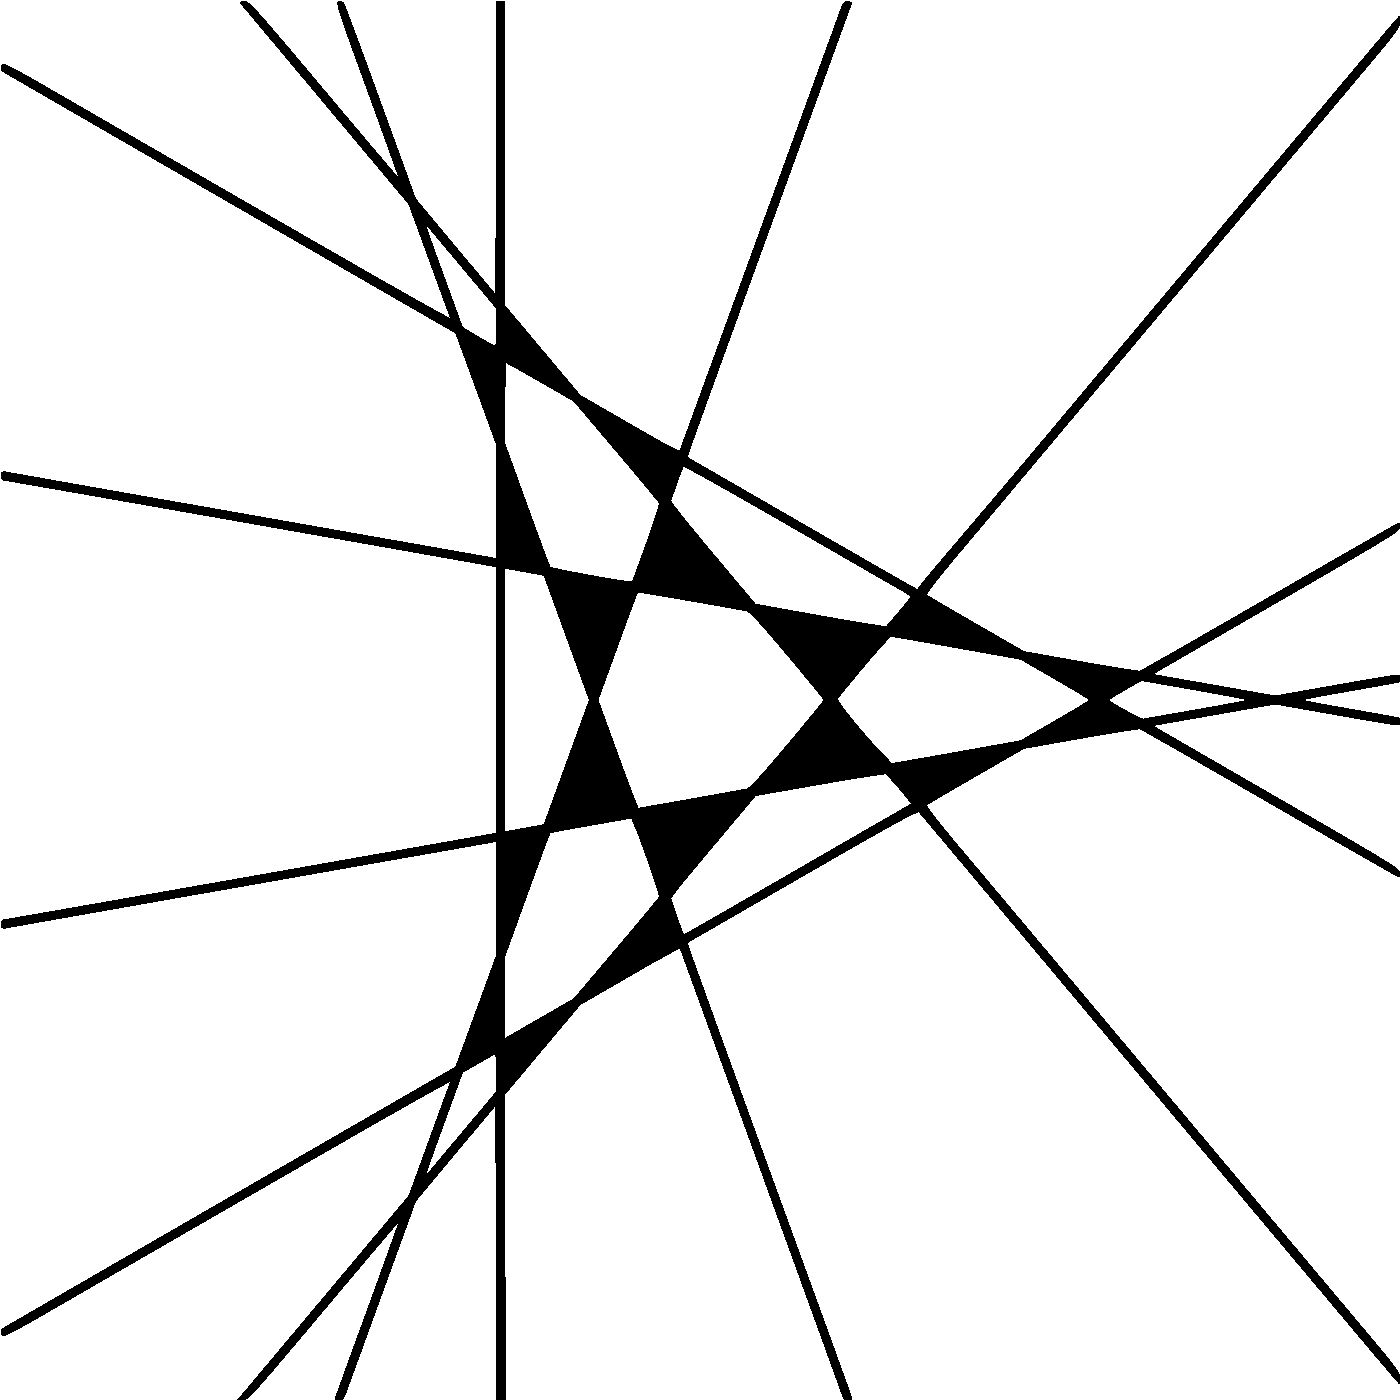
\includegraphics[height=1.5cm]{./../../common/images/vielesing.pdf}
        &
        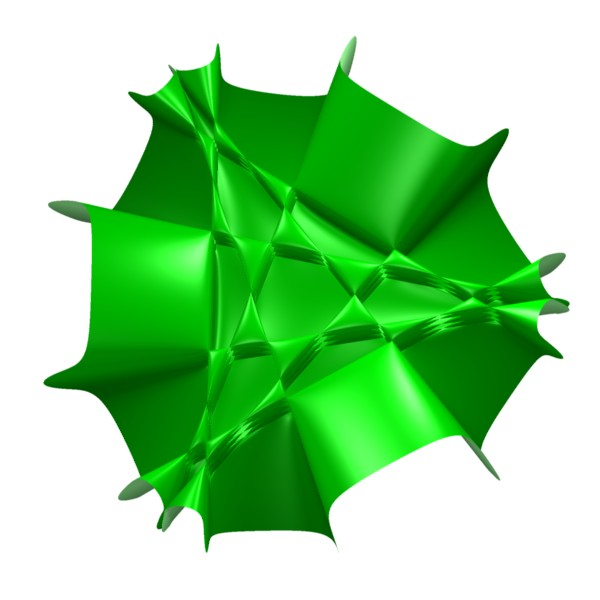
\includegraphics[height=1.5cm]{./../../common/images/p9surface_von_oben}
      \end{tabular}
    \end{center}
\end{surferPage}
